\documentclass{ethz_report}
\usepackage{listings}
\usepackage{color}
\usepackage{caption}
\usepackage{subcaption}


\definecolor{codegreen}{rgb}{0,0.6,0}
\definecolor{codegray}{rgb}{0.5,0.5,0.5}
\definecolor{codepurple}{rgb}{0.58,0,0.82}
\definecolor{backcolour}{rgb}{1,1,1}

\lstdefinestyle{mystyle}{
    backgroundcolor=\color{backcolour},
    commentstyle=\color{codegreen},
    keywordstyle=\color{magenta},
    numberstyle=\tiny\color{codegray},
    stringstyle=\color{codepurple},
    basicstyle=\ttfamily,
    breakatwhitespace=false,
    breaklines=true,
    captionpos=b,
    keepspaces=true,
    numbers=left,
    numbersep=5pt,
    showspaces=false,
    showstringspaces=false,
    showtabs=false,
    tabsize=4,
    frame=lines
}
\lstset{style=mystyle}

\title{Exercise 10 - Image Categorization}
\subject{Computer Vision}
\author{Alberto Montes}
\email{malberto@student.ethz.ch}
\date{\today}

\begin{document}
\maketitle

\section*{Local Feature Extraction}

To extract the local features for each image, first it requires to implement the function to extract the grid points positions for each image.
The implementation is on Listing~\ref{lst:grid_points} where the coordinates of the grid points are found and returned.

\lstinputlisting[language=MATLAB, caption=\texttt{grid\_points.m}, label={lst:grid_points}]{../code/grid_points.m}

The next step is for each of the points of the grid at each image, compute the Histogram of oriented Gradients for $4 \times 4$ grid pixels. The implementation is in Listing~\ref{lst:descriptors_hog} where for each points the descriptor is computed and also the patch of each descriptor is returned.

\lstinputlisting[language=MATLAB, caption=\texttt{descriptors\_hog.m}, label={lst:descriptors_hog}]{../code/descriptors_hog.m}

\section*{Codebook Construction}

Once with the descriptors and patches extracted for each image, is time to construct the codebook.
To do so, a k-means cluster algorithm is run to obtain an specific number of clusters centers to build the codebook. For the implementation, the codebook size its fixed in 200 codes.

For the k-means algorithm implementation first requires to implement the \texttt{findnn} (Listing~\ref{lst:findnn}) function which find to each descriptor the other ones which are closest.
With this function, the k-means algorithm has been implemented as shown in Listing~\ref{lst:kmeans}.

\lstinputlisting[language=MATLAB, caption=\texttt{findnn.m}, label={lst:findnn}]{../code/findnn.m}

\lstinputlisting[language=MATLAB, caption=\texttt{kmeans.m}, label={lst:kmeans}]{../code/kmeans.m}

Finally the whole pipeline of creating the codebook is coded in Listing~\ref{lst:create_codebook}.
The pipeline iterates over all the images and for each on first convert it to gray scale, then obtain the grid points coordinates with the \texttt{grid\_points} function. Then obtain the descriptor for each of this points and the image patch using the \texttt{descriptors\_hog} function.
Finally with all the image's descriptors, cluster them with the \texttt{kmeans} algorithm and obtain the cluster centers as classification codebook. The whole pipeline implementation is on Listing~\ref{lst:create_codebook}.

\lstinputlisting[language=MATLAB, caption=\texttt{create\_codebook.m}, label={lst:create_codebook}]{../code/create_codebook.m}

For the training data given with the assignment, and computing a codebook with size 200, the visualization of the codebook is on Figure~\ref{fig:visualize_codebook} where the patches of the closest descriptors to the codebook cluster's centers are plot.

\begin{figure}[h]
    \centering
    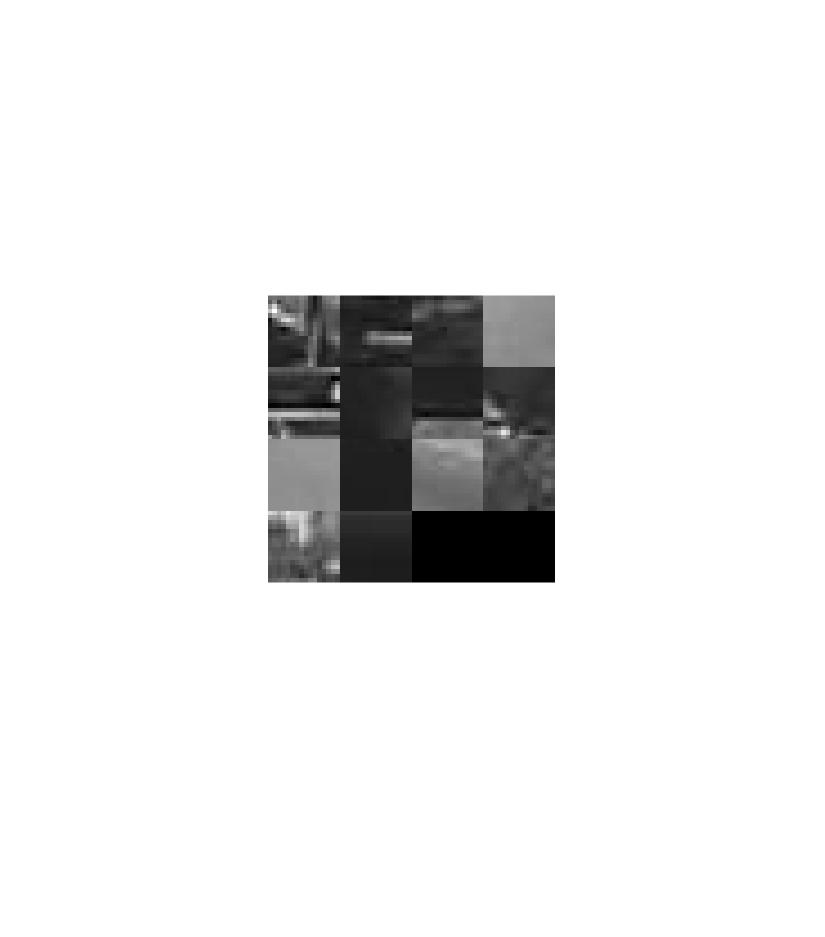
\includegraphics[width=1\linewidth]{images/visualize_codebook}
    \caption{Visualization of the codebook for $K=200$.}
    \label{fig:visualize_codebook}
\end{figure}

\section*{Bag-of-Words Image Representation}

Once the codebook has been defined, for each image is extracted a bunch of descriptors which each one will be match to one of the codebook's code or visual word.
The purpose of the bag-of-words is to represent an image as an histogram of the visual words appearing on it, and with this histogram then perform a classification.
To do so, first the \texttt{bow\_histogram} function has been implemented (in Listing~\ref{lst:bow_histogram}) which for each image given extract the histogram of visual words, given the codebook previously found.

\lstinputlisting[language=MATLAB, caption=\texttt{bow\_histogram.m}, label={lst:bow_histogram}]{../code/bow_histogram.m}

To perform a classification, is necessary to precompute this BoW histograms to all the training examples and store to further classify the test dataset. This is performed in the function \texttt{create\_bow\_histogram} on Listing~\ref{lst:create_bow_histograms}.

\lstinputlisting[language=MATLAB, caption=\texttt{create\_bow\_histograms.m}, label={lst:create_bow_histograms}]{../code/create_bow_histograms.m}

\section*{Nearest Neighbor Classification}

With all the Bag of Words computed for the training samples and also for the testing samples, two methods to classify whether in an image there is a car or not are proposed.
The first method consist on the Nearest Neighbor where for each test samples is computed the distance of the BoW to each of the training samples and the class of the closest distance is returned. The implementation is on Listing~\ref{lst:bow_recognition_nearest} which it has been very easy to code.

\lstinputlisting[language=MATLAB, caption=\texttt{bow\_recognition\_nearest.m}, label={lst:bow_recognition_nearest}]{../code/bow_recognition_nearest.m}

The result of the implementation with the default value of codebook size is a $76.76\%$ accuracy detecting cars.

\section*{Bayesian Classification}

The second classification method proposed consist on a Bayesian Classification. On this method, for each of the features of each image, the prior distributions is found considering that it follows a normal distribution.
So with the training data the $P(hist|car)$ and $P(hist|!car)$ are computed and considering that $P(car)=P(!car)=0.5$, to classify each image, only is necessary to evaluate $log[P(hist|car)]$ and $log[P(hist|!car)]$. The logarithmic is used for numerical stability, so the implementation is listed in Listing~\ref{lst:bow_recognition_bayes}.

\lstinputlisting[language=MATLAB, caption=\texttt{bow\_recognition\_bayes.m}, label={lst:bow_recognition_bayes}]{../code/bow_recognition_bayes.m}

The result of the implementation with the default value of codebook size is a $70.70\%$ accuracy detecting cars.

\section*{Results and Conclusions}

To go further, the classification has been performed for different codebook sizes, going from 10, to 300. Between 20 and 50 has been observed the best results using Bayes and Nearest Neighbors classifiers achieving more than $95\%$ of accuracy. As the codebook size increases, the performance of both classifiers decreases due to the fact that as bigger the codebook, more combinations of BoW and with an small dataset (only 100 training instances) the precision at the time to classify decreases.

\begin{table}
    \centering
    \begin{tabular}{ | c | c | c | }
        \hline
        \textbf{Size Codebook} & \textbf{Nearest Neighbor} & \textbf{Bayesian} \\
        \hline \hline
        10 & 50.50\% & 50.50\% \\
        20 & 93.94\% & \textbf{98.99\%} \\
        50 & \textbf{96.97\%} & 90.90\% \\
        100 & 86.86\% & 83.83\% \\
        150 & 81.81\% & 81.81\% \\
        200 & 76.76\% & 70.70\% \\
        250 & 64.64\% & 66.66\% \\
        300 & 65.65\% & 62.62\% \\
        \hline
    \end{tabular}
    \caption{Results for different codebook sizes.}
    \label{tab:results}
\end{table}

In the Figure~\ref{fig:visualize_codebook_best} there are the codebooks of the best codebook sizes for Nearest Neighbor classification and Bayesian classification respectively.

\begin{figure}[h]
    \centering
    \begin{subfigure}[b]{.5\textwidth}
        \centering
        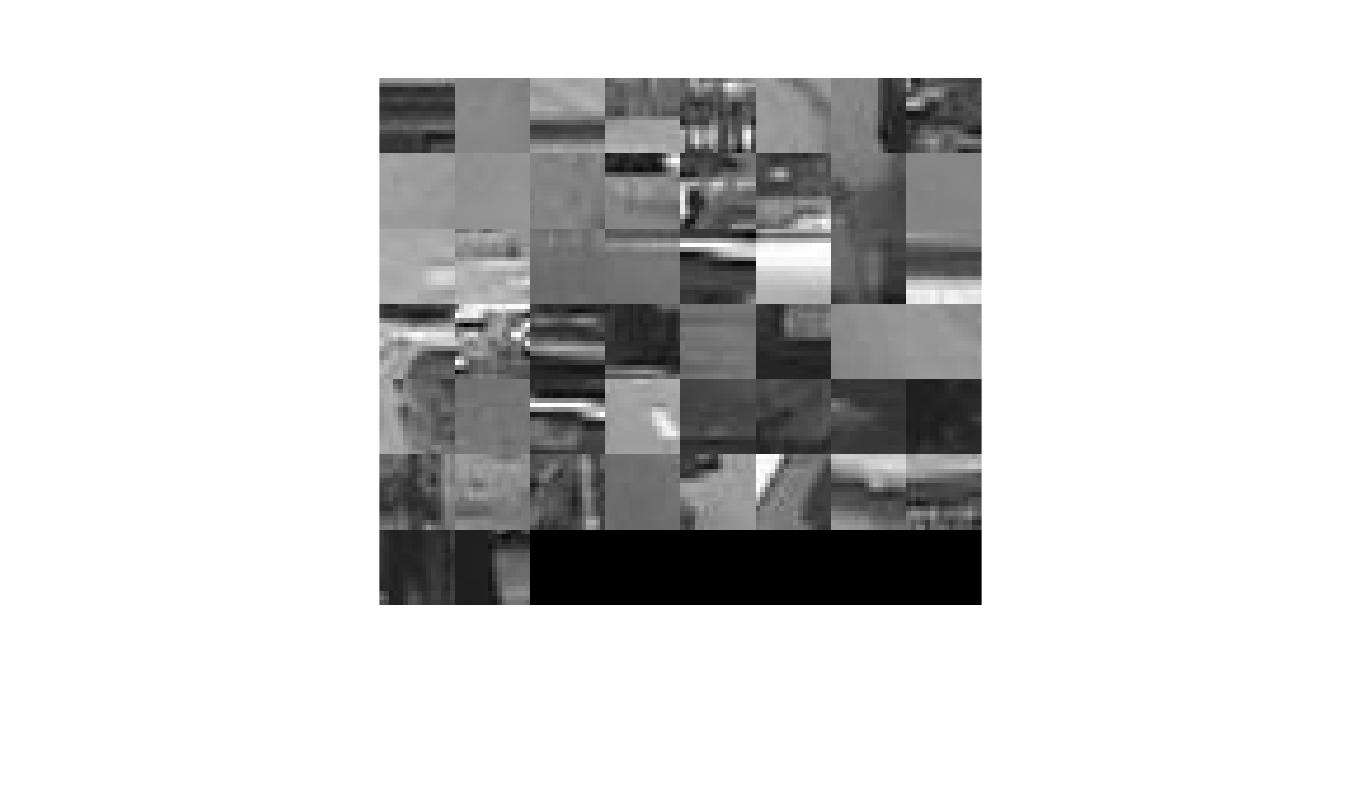
\includegraphics[width=1\linewidth]{images/visualize_codebook_50}
        \subcaption{$K=50$}
    \end{subfigure}%
    \begin{subfigure}[b]{.5\textwidth}
        \centering
        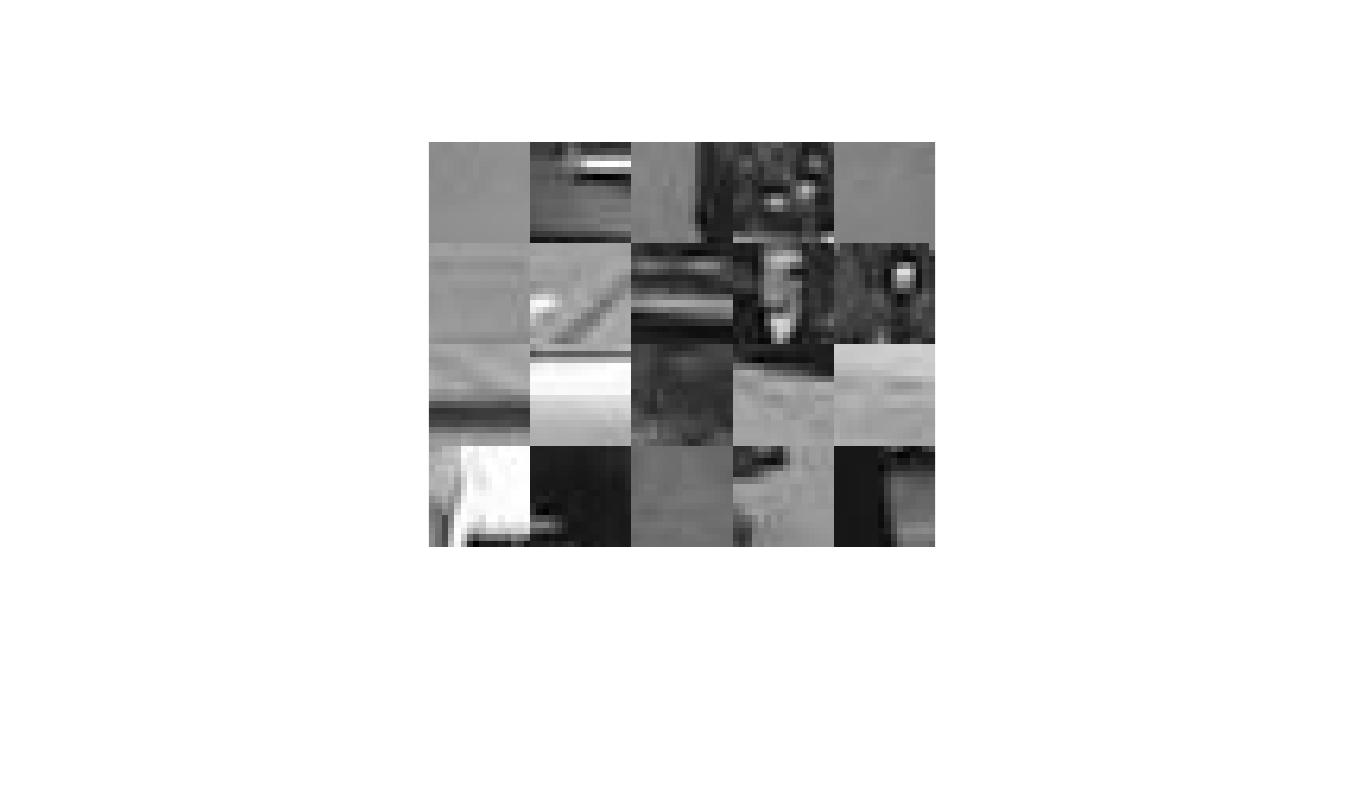
\includegraphics[width=1\linewidth]{images/visualize_codebook_20}
        \subcaption{$K=20$}
    \end{subfigure}
    \caption{Visualize codebook with better classification accuracy.}
    \label{fig:visualize_codebook_best}
\end{figure}

\end{document}
